\documentclass[usenames,dvipsnames,aspectratio=169]{beamer}

\usepackage[utf8]{inputenc}
\usepackage[T1]{fontenc}
\usepackage[magyar]{babel}
\usepackage{indentfirst}
\usepackage{graphicx}
\usepackage{listingsutf8}
\usepackage{textcomp}
\usepackage{eurosym}
\usepackage{mathtools}
\lstset{literate=
  {á}{{\'a}}1 {é}{{\'e}}1 {í}{{\'i}}1 {ó}{{\'o}}1 {ú}{{\'u}}1
  {Á}{{\'A}}1 {É}{{\'E}}1 {Í}{{\'I}}1 {Ó}{{\'O}}1 {Ú}{{\'U}}1
  {à}{{\`a}}1 {è}{{\`e}}1 {ì}{{\`i}}1 {ò}{{\`o}}1 {ù}{{\`u}}1
  {À}{{\`A}}1 {È}{{\'E}}1 {Ì}{{\`I}}1 {Ò}{{\`O}}1 {Ù}{{\`U}}1
  {ä}{{\"a}}1 {ë}{{\"e}}1 {ï}{{\"i}}1 {ö}{{\"o}}1 {ü}{{\"u}}1
  {Ä}{{\"A}}1 {Ë}{{\"E}}1 {Ï}{{\"I}}1 {Ö}{{\"O}}1 {Ü}{{\"U}}1
  {â}{{\^a}}1 {ê}{{\^e}}1 {î}{{\^i}}1 {ô}{{\^o}}1 {û}{{\^u}}1
  {Â}{{\^A}}1 {Ê}{{\^E}}1 {Î}{{\^I}}1 {Ô}{{\^O}}1 {Û}{{\^U}}1
  {œ}{{\oe}}1 {Œ}{{\OE}}1 {æ}{{\ae}}1 {Æ}{{\AE}}1 {ß}{{\ss}}1
  {ç}{{\c c}}1 {Ç}{{\c C}}1 {ø}{{\o}}1 {å}{{\r a}}1 {Å}{{\r A}}1
  {€}{{\EUR}}1 {£}{{\pounds}}1 {ő}{{\H{o}}}1 {ű}{{\H{u}}}1
}
\lstdefinestyle{HTML}{
  language=HTML,
  breaklines=true,
  postbreak=\mbox{\textcolor{red}{$\hookrightarrow$}\space},
  stringstyle=\ttfamily,
  inputencoding=utf8,
  morekeywords={header, time, nav, main, article, section, aside, role, 
    footer, details, open, summary, srcdoc, list, datalist, placeholder, 
    pattern, required, min, max, step, enctype, formaction, formmethod, 
    formnovalidate, formtarget, output}
}
\usepackage{hyperref}
\usepackage{attachfile}
\usepackage{multirow}
% Navigációs pöttyök hozzáadása subsection nélküli fejezetekhez
\usepackage{remreset}
\makeatletter
\@removefromreset{subsection}{section}
\makeatother
\setcounter{subsection}{1}
%%%%%
\attachfilesetup{color={1.0 0.6 0.0},author={HFM},description={Kattintson duplán a minta %
megtekintéséhez!},icon=Paperclip}
\definecolor{kiemelesszin}{rgb}{0.6,0.0,0.0}
\definecolor{kiemelesszinZ}{rgb}{0.0,0.6,0.0}
\definecolor{kiemelesszinN}{RGB}{196,127,0}
\definecolor{hivatkozasszin}{rgb}{0.0,0.0,0.75}
\newcommand{\kiemel}[1]{{\color{kiemelesszin}#1}}
\newcommand{\kiemelZ}[1]{{\color{kiemelesszinZ}#1}}
\newcommand{\kiemelN}[1]{{\color{kiemelesszinN}#1}}
\newcommand{\hiv}[1]{{\color{hivatkozasszin}#1}}
\frenchspacing
\usetheme[compress]{Berlin}

\title[Web technológiák - HTML]{Web-technológia}
\subtitle{Cascading Style Sheets}
\author{Dr. Hatwagner F. Miklós}
\institute{Széchenyi István Egyetem, Győr}
\date{\hiv{\href{https://github.com/wajzy/GKxB\_INTM049.git}{https://github.com/wajzy/GKxB\_INTM049.git}}\\ \today}

\begin{document}

% initial, inherit általános értékekről írni kellene valamit, valahol!
% diaszámokat frissíteni kell, mert csomó helyre közbeszúrtam valamit

%1
\begin{frame}[plain]
  \titlepage
  \begin{picture}(0,0)
    \put(50,-0){\hbox{
\includegraphics[scale=1]{../common/sze_logo.pdf}}}
    \put(205,-11){\hbox{
\includegraphics[scale=.8]{../common/it_logo.pdf}}}
  \end{picture}
\end{frame}

\section{Alapok}

%\subsection{Előnyök}

%2
\begin{frame}
  CSS: Cascading Style Sheets
  \begin{itemize}
    \item $\approx$ lépcsőzetes/sorba kapcsolt stíluslapok
    \item \emph{formázás, megjelenés} leírásának elválasztása a \emph{tartalomtól} (HTML), előnyei:
    \begin{itemize}
      \item külön fájlban tárolható, ami több weboldalhoz is használható, így csökken az összesített kódméret, 
      \item egységessé válik ezen oldalak megjelenése,
      \item egymástól függetlenül, egyidejűleg lehet szerkeszteni a formát és a tartalmat,
      \item gyorsabban módosítható a megjelenés, mert csak egy helyen kell változtatni,
      \item hatékonyabbá válik a gyorstárazás,
    \end{itemize}
    \item különféle médiára eltérő formázás lehetséges (pl. képernyő, nyomtatás)
    \item \hiv{\href{http://www.csszengarden.com/}{a CSS ereje}}
    \item \hiv{\href{https://www.w3.org/Style/CSS/learning.en.html}{hivatalos W3C oldal}}
  \end{itemize}
\end{frame}

%\subsection{Formázás HTML elemekkel és CSS-sel}

%3
\begin{frame}
  \small
  \begin{alertblock}{Elavult módszer (\textattachfile{htmlFormazas.html}{htmlFormazas.html})}
    \lstinputlisting[style=HTML,numbers=left]{htmlFormazas.html}
  \end{alertblock}
\end{frame}

%4
\begin{frame}
  \scriptsize
  \begin{exampleblock}{Formázás CSS-sel (\textattachfile{cssFormazas.html}{cssFormazas.html})}
    \lstinputlisting[style=HTML,linerange={3-10},numbers=left,firstnumber=3]{cssFormazas.html}
  \end{exampleblock}
  \begin{exampleblock}{Formázás CSS-sel (\textattachfile{cssFormazas.css}{cssFormazas.css})}
    \lstinputlisting[style=HTML,numbers=left]{cssFormazas.css}
  \end{exampleblock}
\end{frame}

%\subsection{Szintaktika}

%5
\begin{frame}[fragile]
  \begin{columns}[c]
    \column{0.5\textwidth}
      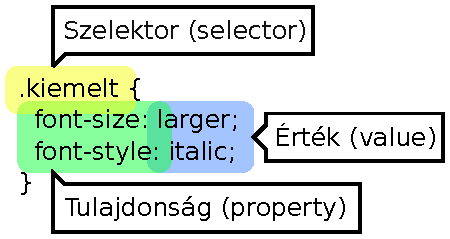
\includegraphics[scale=0.75]{szintakszis.pdf}\\
      \begin{block}{Deklaráció sablonja}
      \vspace{-0.5cm}
\begin{verbatim}
szelektor {
  tulajdonság1: érték(ek);
  tulajdonság2: érték(ek);
  ...
  tulajdonságN: érték(ek);
}
\end{verbatim}
      \vspace{-0.4cm}
      \end{block}
    \column{0.5\textwidth}
      \begin{description}[m]
        \item[Szelektor] \hfill \\ Mit akarunk formázni?
        \item[Tulajdonság] \hfill \\ Milyen tulajdonságán változtassunk?
        \item[Érték] \hfill \\ Milyen legyen az új állapot?
      \end{description}
  \end{columns}
  
\end{frame}

%6
\begin{frame}
  Megjegyzések a CSS-ben:
  \begin{itemize}
    \item \texttt{/* megjegyzes */}
    \item végleges kódból célszerű elhagyni
    \item Lehet több soros is
  \end{itemize} 
  \hiv{\href{https://jigsaw.w3.org/css-validator/}{CSS ellenőrző}}
\end{frame}

%\subsection{Szelektorok}

%7
\begin{frame}
  \begin{description}[m]
    \item[HTML elem neve] \hfill \\ \texttt{p \{ font-style: italic; \}}
    \item[Egyedi azonosító (\texttt{id} attribútum) alapján] \hfill \\ 
      \texttt{\#lablec \{ font-size: 10pt; \}}\\
      Az \texttt{id} nem kezdődhet számjegy karakterrel!
    \item[Univerzális szelektor, mindenre illeszkedik] \hfill \\ \texttt{* \{ font-size: smaller; \}}
  \end{description}
\end{frame}

%8
\begin{frame}
  \begin{description}[m]
    \item[Osztály (\texttt{class} attribútum alapján)] \hfill \\ 
      \texttt{*.kisbetus \{ font-size: small; \} /* bármilyen HTML elemhez */} \\
      \texttt{.kisbetus \{ font-size: small; \} /* bármilyen HTML elemhez, rövid alak */}\\
      \texttt{p.voros \{ color: red; \} /* csak adott (pl. <p>) HTML elemhez */}\\
      A \texttt{class} értéke nem kezdődhet számjeggyel, de lehet egyszerre több, szóközzel elválasztott értéke: \\
      \texttt{<p class="kisbetus voros">Apróbetűs piros bekezdés</p>}
    \item[Elemek csoportosítása] \hfill \\ \texttt{h1, h2, h3 \{ font-family: Arial; \}}
  \end{description}
\end{frame}

%9
\begin{frame}
  \begin{exampleblock}{\textattachfile{egyszeruSzelektor1.html}{egyszeruSzelektor1.html}}
    \scriptsize
    \lstinputlisting[style=HTML,linerange={3-13},numbers=left,firstnumber=3]{egyszeruSzelektor1.html}
  \end{exampleblock}
\end{frame}

%10
\begin{frame}
  \begin{exampleblock}{\textattachfile{egyszeruSzelektor1.html}{egyszeruSzelektor1.html}}
    \scriptsize
    \lstinputlisting[style=HTML,linerange={14-15},numbers=left,firstnumber=14]{egyszeruSzelektor1.html}
  \end{exampleblock}
\end{frame}

%11
\begin{frame}
  \begin{exampleblock}{\textattachfile{egyszeruSzelektor1.css}{egyszeruSzelektor1.css}}
    \scriptsize
    \lstinputlisting[style=HTML,numbers=left]{egyszeruSzelektor1.css}
  \end{exampleblock}
  \begin{center}
    
\includegraphics[width=.9\textwidth]{egyszeruSzelektor1.png}
  \end{center}
\end{frame}

%_
\begin{frame}
  Egy elembe tetszőleges mélységben beágyazott másik elemek kiválasztása
  \begin{columns}[c]
    \column{0.66\textwidth}
      \begin{exampleblock}{\textattachfile{leszarmazott.html}{leszarmazott.html}}
        \footnotesize
        \lstinputlisting[style=HTML,linerange={7-7},numbers=left,firstnumber=7]{leszarmazott.html}
        \lstinputlisting[style=HTML,linerange={11-18},numbers=left,firstnumber=11]{leszarmazott.html}
      \end{exampleblock}
    \column{0.3\textwidth}
      
\includegraphics[width=\textwidth]{leszarmazott.png}
  \end{columns}
\end{frame}

%_
\begin{frame}
  Egy elembe közvetlenül beágyazott gyermek elemek kiválasztása
  \begin{columns}[c]
    \column{0.66\textwidth}
      \begin{exampleblock}{\textattachfile{gyermek.html}{gyermek.html}}
        \footnotesize
        \lstinputlisting[style=HTML,linerange={7-7},numbers=left,firstnumber=7]{gyermek.html}
        \lstinputlisting[style=HTML,linerange={11-18},numbers=left,firstnumber=11]{gyermek.html}
      \end{exampleblock}
    \column{0.3\textwidth}
      
\includegraphics[width=\textwidth]{gyermek.png}
  \end{columns}
\end{frame}

%_
\begin{frame}
  Egy elemet közvetlenül követő testvér elem kiválasztása
  \begin{columns}[c]
    \column{0.66\textwidth}
      \begin{exampleblock}{\textattachfile{testver.html}{testver.html}}
        \footnotesize
        \lstinputlisting[style=HTML,linerange={7-7},numbers=left,firstnumber=7]{testver.html}
        \lstinputlisting[style=HTML,linerange={11-19},numbers=left,firstnumber=11]{testver.html}
      \end{exampleblock}
    \column{0.3\textwidth}
      
\includegraphics[width=\textwidth]{testver.png}
  \end{columns}
\end{frame}

%_
\begin{frame}
  Egy elemet közvetlenül követő összes testvér kiválasztása
  \begin{columns}[c]
    \column{0.66\textwidth}
      \begin{exampleblock}{\textattachfile{testver2.html}{testver2.html}}
        \footnotesize
        \lstinputlisting[style=HTML,linerange={7-7},numbers=left,firstnumber=7]{testver2.html}
        \lstinputlisting[style=HTML,linerange={11-19},numbers=left,firstnumber=11]{testver2.html}
      \end{exampleblock}
    \column{0.3\textwidth}
      
\includegraphics[width=\textwidth]{testver2.png}
  \end{columns}
\end{frame}

%_
\begin{frame}
  Látszólagos osztályok (pseudo-class): egy elem adott állapota esetén alkalmazandó formázása, 
  \hiv{\href{https://developer.mozilla.org/en-US/docs/Web/CSS/Pseudo-classes}{referencia}}
  \vfill
  Az egér alatti elem kiválasztása
  \begin{columns}[c]
    \column{0.66\textwidth}
      \begin{exampleblock}{\textattachfile{hover.html}{hover.html}}
        \footnotesize
        \lstinputlisting[style=HTML,linerange={7-7},numbers=left,firstnumber=7]{hover.html}
        \lstinputlisting[style=HTML,linerange={11-11},numbers=left,firstnumber=11]{hover.html}
      \end{exampleblock}
    \column{0.3\textwidth}
      
\includegraphics[width=\textwidth]{hover1.png}
      \vfill
      
\includegraphics[width=\textwidth]{hover2.png}
  \end{columns}
\end{frame}

%_
\begin{frame}
  Azon elemek kiválasztása, melyek a szülőjük első gyermekei
  \begin{columns}[c]
    \column{0.66\textwidth}
      \begin{exampleblock}{\textattachfile{firstchild.html}{firstchild.html}}
        \scriptsize
        \lstinputlisting[style=HTML,linerange={7-7},numbers=left,firstnumber=7]{firstchild.html}
        \lstinputlisting[style=HTML,linerange={10-14},numbers=left,firstnumber=10]{firstchild.html}
      \end{exampleblock}
    \column{0.3\textwidth}
      
\includegraphics[width=\textwidth]{firstchild.png}
  \end{columns}
\end{frame}

%_
\begin{frame}
  Nyelvfüggő beállítások alkalmazása
  \begin{columns}[c]
    \column{0.66\textwidth}
      \begin{exampleblock}{\textattachfile{lang.html}{lang.html}}
        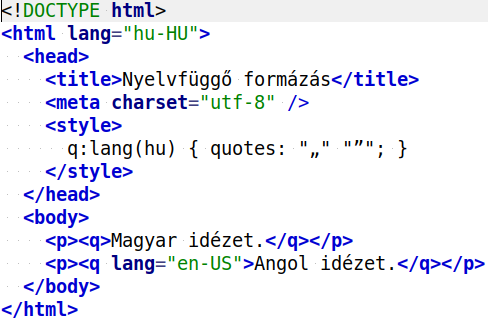
\includegraphics[width=0.7\textwidth]{langhtml.png}
      \end{exampleblock}
    \column{0.3\textwidth}
      
\includegraphics[width=\textwidth]{lang.png}
  \end{columns}
\end{frame}

%_
\begin{frame}
  Adott típus n-edik előfordulása (részleteket ld. később \texttt{nth-child()}-nál)
  \begin{columns}[c]
    \column{0.7\textwidth}
      \begin{exampleblock}{\textattachfile{nthoftype.html}{nthoftype.html}}
        \scriptsize
        \lstinputlisting[style=HTML,linerange={7-7},numbers=left,firstnumber=7]{nthoftype.html}
        \lstinputlisting[style=HTML,linerange={11-16},numbers=left,firstnumber=11]{nthoftype.html}
      \end{exampleblock}
    \column{0.25\textwidth}
      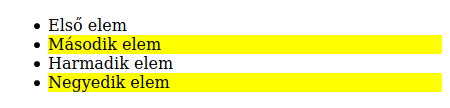
\includegraphics[width=\textwidth]{nthoftype.png}
  \end{columns}
\end{frame}

%ide jöhetnének a mértékegységek
%\subsection{Stílusok forrása}

%12
\begin{frame}
  Háromféle helyen lehet stílusokat megadni:
  \begin{enumerate}
    \item Külső fájlban (\texttt{css} kiterjesztés, \texttt{<link>} elem)
    \item A \texttt{<head>} elembe ágyazott \texttt{<style>} elemben. Csak akkor ajánlott, ha egyetlen HTML fájlt kívánunk formázni ezekkel a stílusokkal.
    \item Soron belül: a HTML elemek \texttt{style} attribútumának értékeként. Ismét \kiemel{keveredik a tartalom a stílussal}, ezért általában \kiemel{nem ajánlott} a használata!
  \end{enumerate}
\end{frame}

%13
\begin{frame}
  \begin{exampleblock}{\textattachfile{egyszeruSzelektor2.html}{egyszeruSzelektor2.html}}
    \footnotesize
    \lstinputlisting[style=HTML,linerange={3-12},numbers=left,firstnumber=3]{egyszeruSzelektor2.html}
    \lstinputlisting[style=HTML,linerange={16-16},numbers=left,firstnumber=16]{egyszeruSzelektor2.html}
  \end{exampleblock}
\end{frame}

%\subsection{Ütközések feloldása}

%14
\begin{frame}
  \begin{itemize}
    \item Ha több előírás is vonatkozik ugyanannak az objektumnak a formázására, elsőként a forrás prioritása dönt (csökkenő sorrendben):
    \begin{enumerate}
      \item soron belüli formázások
      \item külső és belső (\texttt{<link>}, \texttt{<style>} elemek) formázások
      \item böngésző alapértelmezése
    \end{enumerate}
    \item Ha forrás alapján nem lehet különbséget tenni, megvizsgálják a \emph{specifikusságot}.
    \item Ha ez sem segít, a később betöltött szabály felülírja a korábbit.
  \end{itemize}
  
\end{frame}

%15
\begin{frame}
  \begin{exampleblock}{\textattachfile{utkozes1.html}{utkozes1.html}}
    \scriptsize
    \lstinputlisting[style=HTML,linerange={6-13},numbers=left,firstnumber=6]{utkozes1.html}
  \end{exampleblock}
  \begin{columns}[T]
    \column{0.6\textwidth}
      \begin{exampleblock}{\textattachfile{utkozes1.css}{utkozes1.css}}
        \scriptsize
        \lstinputlisting[style=HTML,numbers=left,firstnumber=1]{utkozes1.css}
      \end{exampleblock}
    \column{0.3\textwidth}
      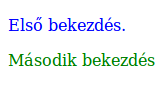
\includegraphics[width=.66\textwidth]{utkozes1.png}
  \end{columns} 
\end{frame}

%16
\begin{frame}
  \begin{exampleblock}{\textattachfile{utkozes2.html}{utkozes2.html}}
    \scriptsize
    \lstinputlisting[style=HTML,linerange={6-13},numbers=left,firstnumber=6]{utkozes2.html}
  \end{exampleblock}
  \begin{columns}[T]
    \column{0.6\textwidth}
      \begin{exampleblock}{\textattachfile{utkozes1.css}{utkozes1.css}}
        \scriptsize
        \lstinputlisting[style=HTML,numbers=left,firstnumber=1]{utkozes1.css}
      \end{exampleblock}
    \column{0.3\textwidth}
      
\includegraphics[width=.66\textwidth]{utkozes2.png}
  \end{columns} 
\end{frame}

%_
\begin{frame}
  Specifikusság meghatározása
  \begin{enumerate}
    \renewcommand{\theenumi}{\Alph{enumi}}
    \item = 1, ha a stílus a \texttt{<style>} attribútumban található, egyébként 0\\(pl. \texttt{<p style="color: red;">...</p>})
    \item = a szelektorban lévő ID attribútumok száma (pl. \texttt{\#bekezdes})
    \item = a szelektorban lévő osztályok, attribútumok és látszólagos osztályok száma\\(pl. \texttt{.bekezdes}, \texttt{a[target="\_blank"]}, \texttt{a:hover})
    \item = az elemnevek és látszólagos elemek száma (pl. \texttt{p}, \texttt{p::first-line})
  \end{enumerate}
  Az univerzális szelektor (\texttt{*}) és ami ebből származik (pl. \texttt{body *}) 0 specifikusságú.
\end{frame}

%_
\begin{frame}
  \begin{center}
    \begin{tabular}{lllll}
    Szelektor & B & C & D & Specifikusság \\ \hline
    \texttt{*} & 0 & 0 & 0 & 0\\
    \texttt{p} & 0 & 0 & 1 & 1\\
    \texttt{div p} & 0 & 0 & 2 & 2\\
    \texttt{ul ol + li} & 0 & 0 & 3 & 3\\
    \texttt{h1 + *[title]} & 0 & 1 & 1 & 11\\
    \texttt{ul ol li.voros} & 0 & 1 & 3 & 13\\
    \texttt{li.voros.szint} & 0 & 2 & 1 & 21\\
    \texttt{\#oszlopfej} & 1 & 0 & 0 & 100
    \end{tabular}
  \end{center}
\end{frame}

%\subsection{Színek}

%17
\begin{frame}
  Számtalan dolognak beállítható a színe CSS tulajdonságokkal, pl.:
  \begin{description}[m]
    \item[\texttt{color}] \hfill \\ Szöveg írásszíne
    \item[\texttt{background-color}] \hfill \\ Háttérszín
  \end{description}
  Szín, mint a tulajdonság értéke megadható:
  \begin{description}[m]
    \item[kulcsszavakkal] \hfill \\ Pl. \texttt{red} (vörös), 
    \texttt{green} (zöld), \texttt{blue} (kék), \texttt{white} (fehér), 
    \texttt{black} (fekete), \dots \\
    \hiv{\href{https://www.w3.org/TR/css-color-3/\#svg-color}%
    {140 szabványos színkód}}
    \item[Hexadecimálisan, RGB összetevőkkel] \hfill \\ Pl. 
    narancsszín: \texttt{\#ff7f00}, ahol \texttt{\#} jelzi a 16-os 
    számrendszerbeli alakot, \texttt{ff} a vörös (\kiemel{R}ed), 
    \texttt{7f} a zöld (\kiemel{G}reen) és \texttt{00} a kék 
    (\kiemel{B}lue) összetevő intenzitása 8 biten előjel nélkül, 
    fixpontosan. Additív színkeverés.
  \end{description}
\end{frame}

%18
\begin{frame}
  \begin{description}[m]
    \item[\texttt{rgb()} függvénnyel] \hfill \\ \texttt{rgb(red, 
    green, blue)}, ahol mindhárom összetevő lehet 0-255 közötti 
    decimális egész, vagy 0-100\%. Pl. \texttt{rgb(255,0,0)} vagy 
    \texttt{rgb(100\%, 0\%, 0\%)} vörös színt eredményez.
    \item[\texttt{rgba()} függvénnyel] \hfill \\ \texttt{rgb(red, 
    green, blue, alpha)}, ahol a színösszetevőket egy 
    átlátszóság érték követi ([0, 1]).
  \end{description}
  \vfill
  \begin{center}
    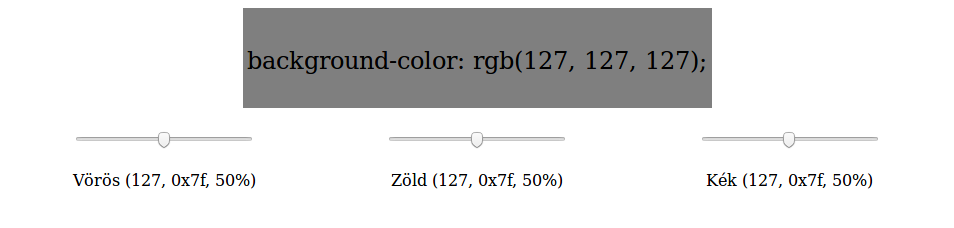
\includegraphics[scale=0.2]{szinek1.png}\\
    \textattachfile{szinek1.html}{szinek1.html}
  \end{center}
\end{frame}

%19
\begin{frame}
  \begin{description}[m]
    \item[\texttt{hsl()} függvénnyel] \hfill \\ \texttt{hsl(hue, 
    saturation, lightness)}, ahol \texttt{hue} az árnyalat, [0, 360] 
    fok közötti elfordulás a színkeréken. Pl. 0$^{\circ}$ a 
    vöröshöz, 120$^{\circ}$ a zöldhöz, 240$^{\circ}$ a kékhez 
    tartozik. \texttt{saturation} a telítettség, százalékban. A 0\% 
    a színinformáció hiányát (szürkeség) jelzi, 100\% a teljes 
    színezettséget. \texttt{lightness} a fényesség, szintén 
    százalékban. A 0\% mindig fekete, a 100\% mindig fehér színt ad.
    \item[\texttt{hsla()} függvénnyel] \hfill \\ A fentiek 
    kiegészülnek átlátszósággal.
  \end{description}
  \vfill
  \begin{center}
    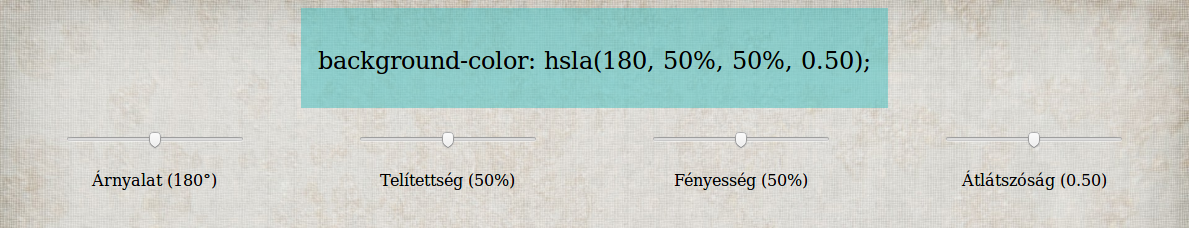
\includegraphics[scale=0.2]{szinek2.png}\\
    \textattachfile{szinek2.html}{szinek2.html}
  \end{center}
\end{frame}

%20
\begin{frame}
  \begin{columns}[c]
    \column{0.5\textwidth}
      Induljon ki a \textattachfile{szinezes.html}{szinezes.html} 
      fájlból! Kapcsolja ezt össze egy külső stíluslappal, majd 
      érje el, hogy a jobb oldali ábrának megfelelő színekben 
      pompázzon! Próbáljon minél több féle szín megadási 
      módszert alkalmazni! Törekedjen a lehető legtömörebb CSS 
      szabályok megalkotására!
    \column{0.5\textwidth}
      \begin{exampleblock}{\textattachfile{szinezes-mo.html}{szinezes-mo.html}, 
        \textattachfile{szinezes-mo.css}{szinezes-mo.css}}
        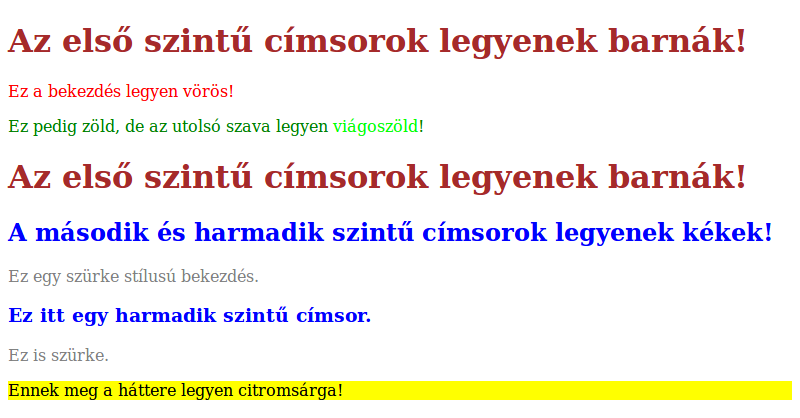
\includegraphics[width=\textwidth]{szinezes-mo.png}
      \end{exampleblock}
  \end{columns} 
\end{frame}

%\subsection{Háttér}

%21
\begin{frame}
  HTML elemek hátterével kapcsolatos tulajdonságok:
  \begin{description}[m]
    \item[\texttt{background-color}] \hfill \\ A háttér színe. 
    Alapértelmezetten \texttt{transparent}, azaz átlátszó.
    \item[\texttt{background-image}] \hfill \\ Háttérkép, amivel 
    alapértelmezés szerint kicsempézi az elem teljes területét 
    (margókat nem). 
    Alapértéke \texttt{none}, nincs háttérkép. Az \texttt{url()} 
    függvény paramétereként adható meg a képfájl, pl. \\
    \texttt{background-color: url("hatter.png");} \\Megadhatók 
    \hiv{\href{https://cssgradient.io/}{színátmenetek}} is.\\
    A szöveg maradjon \kiemel{olvasható} a háttéren!
  \end{description}
\end{frame}

%22
\begin{frame}
  \begin{description}[m]
    \item[\texttt{background-repeat}] \hfill \\ Háttérkép 
    csempézési iránya
    \begin{itemize}
      \item \texttt{repeat} mindkét irányban, túlnyúló részek 
      levágásával, alapértelmezés
      \item \texttt{repeat-x} csak vízszintesen
      \item \texttt{repeat-y} csak függőlegesen
      \item \texttt{no-repeat} csak egyszer, alapértelmezetten a bal 
      felső sarokban
      \item \texttt{round} torzítja a képet a vágás elkerülésére
      \item \texttt{space} csak annyiszor ismétel, ami vágás 
      nélkül elfér, közöttük helyet hagy
    \end{itemize}
    Két érték megadásakor az első a vízszintes, második a 
    függőleges irányra vonatkozik.
  \end{description}
\end{frame}

%23
\begin{frame}
  \begin{center}
    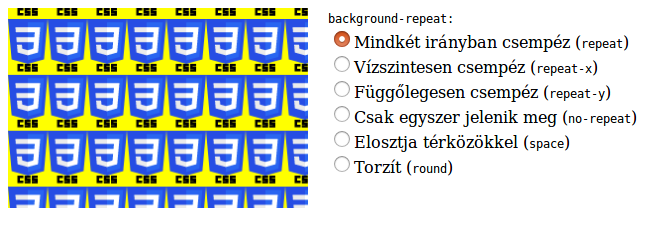
\includegraphics[width=.75\textwidth]{hatter.png}\\
    \textattachfile{hatter.html}{hatter.html}
  \end{center}
\end{frame}

%24
\begin{frame}
  \begin{description}[m]
    \item[\texttt{background-position}] \hfill \\ Igazítás, a 
      \emph{vízszintes} és a \emph{függőleges} pozíciót várja. Ha egyet 
      kap, a másik \texttt{center} lesz.
      \begin{itemize}
        \item Függőlegesen: \texttt{left}, \texttt{center}, 
        \texttt{right}
        \item Vízszintesen: \texttt{top}, \texttt{center}, 
        \texttt{bottom}
        \item Mindkettőnél lehet százelékot, vagy egyéb CSS 
        mértékegységet (pl. képpont) használni. 
      \end{itemize}
  \end{description}
\end{frame}

%25
\begin{frame}
  \begin{exampleblock}{\textattachfile{pozicio1.html}{pozicio1.html}}
    \fontsize{7}{8} \selectfont
    \lstinputlisting[style=HTML,linerange={7-11},numbers=left,firstnumber=7]{pozicio1.html}
    \lstinputlisting[style=HTML,linerange={15-16},numbers=left,firstnumber=15]{pozicio1.html}
    \lstinputlisting[style=HTML,linerange={24-25},numbers=left,firstnumber=24]{pozicio1.html}
    \lstinputlisting[style=HTML,linerange={37-38},numbers=left,firstnumber=37]{pozicio1.html}
    \lstinputlisting[style=HTML,linerange={53-54},numbers=left,firstnumber=53]{pozicio1.html}
  \end{exampleblock}
\end{frame}

%26
\begin{frame}
  \begin{description}[m]
    \item[\texttt{background-attachment}] \hfill \\
      \begin{itemize}
        \item \texttt{scroll} a háttér együtt gördül az oldallal, 
        alapértelmezés
        \item \texttt{fixed} rögzített háttér
        \item \texttt{local} az elem tartalmával együtt gördül a háttér
      \end{itemize}
      \vfill
      A logo mindig a jobb alsó sarokban: 
      \textattachfile{rogzites1.html}{rogzites1.html}\\
      Két bekezdés között kilátszik a háttérben rögzített logo: 
      \textattachfile{rogzites2.html}{rogzites2.html}
  \end{description}
\end{frame}

%27
\begin{frame}
  \begin{description}[m]
    \item[\texttt{background}] \hfill \\ Rövidítés: egy összetett 
    tulajdonsággal sok egyszerű tulajdonság értéke állítható 
    be. \kiemel{Értékek sorrendje rögzített, de tetszőleges 
    számú érték elhagyható!}\\
    \texttt{background: \emph{background-color background-image 
    background-repeat}\\
    \qquad\emph{background-attachment background-position}}
  \end{description}
  \begin{columns}[T]
    \column{0.5\textwidth}
      \begin{exampleblock}{\textattachfile{pozicio1.html}{pozicio1.html}}
        \fontsize{7}{8} \selectfont
        \lstinputlisting[xleftmargin=-1cm,style=HTML,linerange={7-11}]{pozicio1.html}
      \end{exampleblock}
    \column{0.5\textwidth}
      \begin{exampleblock}{\textattachfile{pozicio2.html}{pozicio2.html}}
        \fontsize{7}{8} \selectfont
        \lstinputlisting[xleftmargin=-1cm,style=HTML,linerange={7-10}]{pozicio2.html}
      \end{exampleblock}
  \end{columns} 
\end{frame}

%28
\begin{frame}
  \begin{description}[m]
    \item[\texttt{background-size}] \hfill \\
      \begin{itemize}
        \item \texttt{auto}: Alapértelmezés, eredeti méret.
        \item \emph{szélesség, magasság}: utóbbi elhagyásával 
        \texttt{auto}-t feltételez. Használhatók CSS 
        mértékegységek és százalékok (\kiemel{a szülő elem mérete a 
        100\%}, nem a sajátja!).
        \item \texttt{cover} Addig nyújt és vág, amíg le nem fedi a 
        szülő elem teljes területét.
        \item \texttt{contain} Addig nyújt, amíg egyszer bele nem fér a 
        háttér a szülő elembe.
      \end{itemize}
  \end{description}
  \vfill
  \begin{center}
    
\includegraphics[scale=0.3]{meret.png}\\
    \textattachfile{meret.html}{meret.html}
  \end{center}
\end{frame}

%29
\begin{frame}
  \begin{columns}[c]
    \column{0.5\textwidth}
      \footnotesize
      Induljon ki a \textattachfile{rogzites2.html}{rogzites2.html} 
      fájlból, és alakítsa át a jobb oldali ábrának megfelelően!
      \begin{itemize}
        \item Az írásszín legyen világos szürke!
        \item A teljes oldal háttere legyen kék (RGB-összetevők: 0, 
        145 és 190)!
        \item A \texttt{<div>} elem háttereként állítsa be a 
        \textattachfile{HTML5sticker.png}{HTML5sticker.png} fájl!
        \item Ennek helyzete ne függjön a görgetéstől!
        \item Helyezze el azt a képernyő közepén!
        \item A képet méretezze aránytartó módon úgy, hogy éppen 
        kitöltse a rendelkezésre álló helyet!
        \item Próbálja mindezt a lehető legkevesebb CSS tulajdonság 
        felhasználásával elérni!
      \end{itemize}
    \column{0.5\textwidth}
      \begin{exampleblock}{\textattachfile{rogzites3-mo.html}{rogzites3-mo.html}, \textattachfile{HTML5sticker.png}{HTML5sticker.png}}
        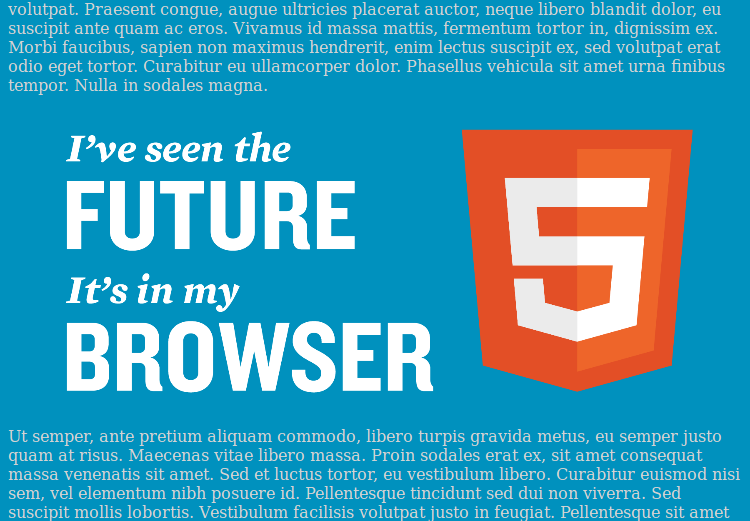
\includegraphics[width=\textwidth]{rogzites3-mo.png}
      \end{exampleblock}
  \end{columns} 
\end{frame}

%\subsection{Dobozmodell}

%30
\begin{frame}
  \begin{columns}[c]
    \column{0.5\textwidth}
      Minden HTML elemet egy \emph{doboznak} tekintünk. Ezek szerkezete belülről kifelé:
      \begin{itemize}
        \item Az elem tartalma (szöveg, kép, \dots)
        \item Kitöltés (\texttt{padding}; átlátszó)
        \item Szegély (\texttt{border})
        \item Margó (\texttt{margin}; átlátszó)
      \end{itemize}
      \vfill
      Megjegyzések
      \begin{itemize}
        \item A szélesség (\texttt{width}) és magasság (\texttt{height}) 
      tulajdonságok a tartalmi rész méreteire vonatkoznak.
        \item Soron belüli elemek méretét a böngésző határozza 
        meg, nem méretezhetőek át.
      \end{itemize}
    \column{0.5\textwidth}
      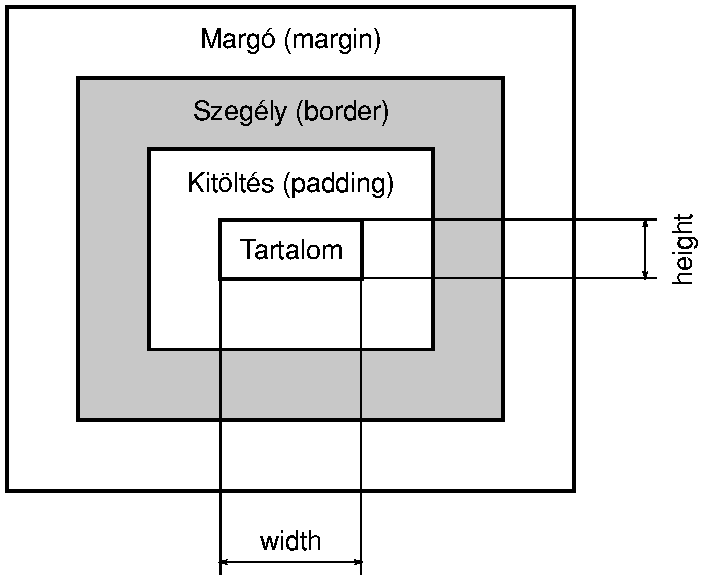
\includegraphics[width=\textwidth]{doboz.pdf}
  \end{columns} 
\end{frame}

%31
\begin{frame}
  \begin{columns}[c]
    \column{0.45\textwidth}
      \begin{exampleblock}{\textattachfile{dobozMeret.html}{dobozMeret.html}}
        \tiny
        \lstinputlisting[style=HTML,linerange={7-18},numbers=left,firstnumber=7]{dobozMeret.html}
      \end{exampleblock}
    \column{0.55\textwidth}
      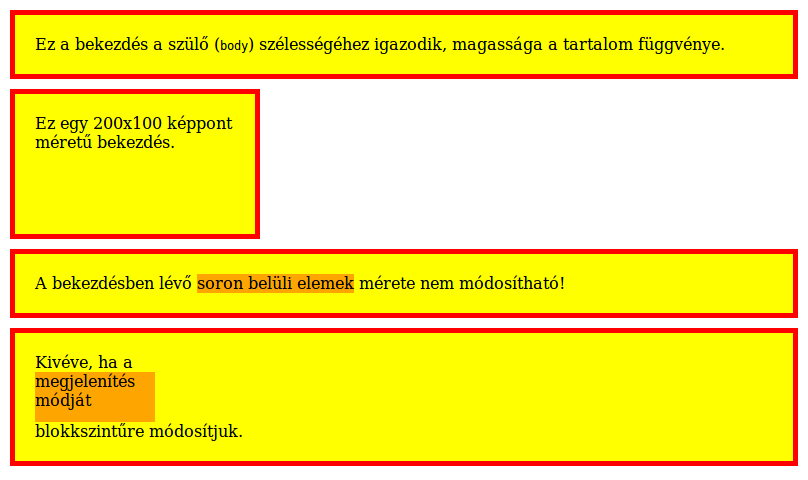
\includegraphics[width=0.9\textwidth]{dobozMeret.png}
  \end{columns}
  \begin{exampleblock}{\vspace*{-3ex}}
    \tiny
    \lstinputlisting[style=HTML,linerange={22-25},numbers=left,firstnumber=22]{dobozMeret.html}
  \end{exampleblock}
\end{frame}

%32
\begin{frame}
\begin{columns}[c]
  \column{0.5\textwidth}
    Mit számol bele a böngésző a méret (\texttt{width}, 
    \texttt{height}) adatokba? $\to$ \texttt{box-sizing}
    \begin{description}[m]
      \item[\texttt{content-box}] \hfill \\ 
        Csak a tartalom méretét
      \item[\texttt{border-box}] \hfill \\ 
        Tartalom + kitöltés + szegély
    \end{description}
  \column{0.5\textwidth}
    \begin{center}
      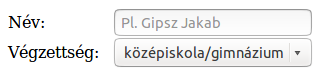
\includegraphics[scale=0.5]{meretezes.png}
    \end{center}
    \begin{exampleblock}{\textattachfile{meretezes.html}{meretezes.html}}
      \scriptsize
      \lstinputlisting[style=HTML,linerange={11-17},numbers=left,firstnumber=11]{meretezes.html}
    \end{exampleblock}
\end{columns} 
  
\end{frame}

%\subsection{Szegélyek}

%37
\begin{frame}
  A szegélyeknek állítható a
  \begin{itemize}
    \item stílusa (\texttt{border-style}),
    \item szélessége (\texttt{border-width}), és a 
    \item színe (\texttt{border-color}).
  \end{itemize}
  Megjegyzések:
  \begin{itemize}
    \item Utóbbi kettő csak a stílus beállítása esetén működik.
    \item Minden paraméter állítható külön az egyes oldalakra is.
  \end{itemize}
\end{frame}

%38
\begin{frame}
  \begin{exampleblock}{\textattachfile{szegelyek1.html}{szegelyek1.html}}
    \scriptsize
    \lstinputlisting[style=HTML,linerange={14-17},numbers=left,firstnumber=14]{szegelyek1.html}
  \end{exampleblock}
  \begin{columns}[T]
    \column{0.25\textwidth}
      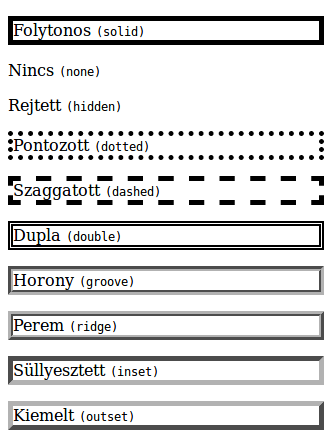
\includegraphics[scale=0.25]{szegelyek1.png}
    \column{0.7\textwidth}
      Oldalankénti szegélystílusok megadhatók:
      \begin{itemize}
        \item 1-4 érték megadásával, pl. \\ \texttt{border-style: dotted dashed solid none;}
        \item Oldalakra vonatkozó tulajdonságokkal: 
        \texttt{border-*-style}, ahol \texttt{*} helyén állhat 
        \texttt{top}, \texttt{right}, \texttt{bottom}, \texttt{left}.
      \end{itemize}
  \end{columns} 
\end{frame}

%39
\begin{frame}
  \begin{columns}[c]
    \column{0.6\textwidth}
      Ha a \texttt{boder-style}-nak
      \begin{description}[m]
        \item[1 értéke van] \hfill \\ \texttt{felül-jobb-alul-bal} (minden 
        oldalra ugyanazt a stílust állítja)
        \item[2 értéke van] \hfill \\ \texttt{felül-alul jobb-bal}
        \item[3 értéke van] \hfill \\ \texttt{felül jobb-bal alul}
        \item[4 értéke van] \hfill \\ \texttt{felül jobb alul bal} (óramutató 
        járása szerint)
      \end{description}
      \vfill
      Hasonlóképpen lehet oldalanként szabályozni a margókat és 
      kitöltéseket is.
    \column{0.35\textwidth}
      \begin{center}
        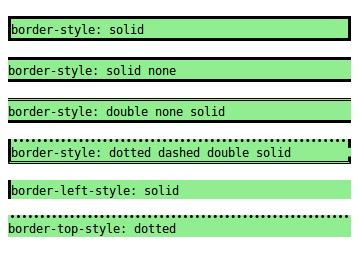
\includegraphics[width=\textwidth]{szegelyek2.png} \\
        \textattachfile{szegelyek2.html}{szegelyek2.html}
      \end{center}
  \end{columns} 
\end{frame}

%40
\begin{frame}
  \begin{columns}[c]
    \column{0.5\textwidth}
      Ha táblázatok szomszédos cellái közös, de eltérő stílusú szegélyeket 
      használnak, akkor
      \begin{description}[m]
        \item[\texttt{none}] \hfill \\ 
          ha a szomszédnak be van állítva a szegélye, az fog megjelenni
        \item[\texttt{hidden}] \hfill \\ 
          még ha be is van állítva a szomszéd szegélye, akkor sem 
          fog megjelenni
      \end{description}
    \column{0.5\textwidth}
      \begin{center}
        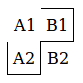
\includegraphics[scale=0.5]{szegelyek3.png}
      \end{center}
      \begin{exampleblock}{\textattachfile{szegelyek3.html}{szegelyek3.html}}
        \scriptsize
        \lstinputlisting[style=HTML,linerange={21-21},numbers=left,firstnumber=21]{szegelyek3.html}
        \lstinputlisting[style=HTML,linerange={26-26},numbers=left,firstnumber=26]{szegelyek3.html}
      \end{exampleblock}
  \end{columns} 
\end{frame}

%41
\begin{frame}
  Rövidítések
  \begin{description}[m]
    \item[\texttt{border: width style color}] \hfill \\ 
      Minden oldalon beállítja a szegély szélességét, stílusát, színét.
    \item[\texttt{border-*: width style color}] \hfill \\ 
      A \texttt{*} lehet \texttt{top}, \texttt{right}, \texttt{bottom} 
      és \texttt{left}; csak ezekre állítja a fenti három tulajdonságot.
  \end{description}
\end{frame}

%\subsection{Margók}

%38
\begin{frame}
  A margók mindig átlátszók, csak a szélességük állítható:
  \begin{itemize}
    \item 1-4 érték megadásával, pl.\\
    \texttt{margin: 10px 20px 30px 40px;}\\
    (Fent, jobbra, lent, balra; további esetek mint \texttt{border-style}-nál.)
    \item Oldalakra vonatkozó tulajdonságokkal:\\
      \texttt{margin-*}, ahol \texttt{*} helyén állhat 
      \texttt{top}, \texttt{right}, \texttt{bottom}, \texttt{left}.
  \end{itemize}
\end{frame}

%39
\begin{frame}
  A margó szélessége lehet:
  \begin{itemize}
    \item \texttt{auto}: a tartalom által fel nem használt helyet felosztja egyenlően a bal és jobb oldal közt $\to$ középre igazít
    \item \texttt{inherit}: a befoglaló, szülő elem beállításait örökli
    \item CSS mértékegységgel (pl. \texttt{px}, \texttt{cm}) adott
    \item \texttt{\%}: a szülő elem méretének százaléka
  \end{itemize}
  \vfill
  Negatív értékek is használhatók.
\end{frame}

%40
\begin{frame}
  A blokkok felső és alsó margói időnként összeolvadnak, és a kettő közül csak a nagyobb marad meg:
  \begin{itemize}
    \item szülő szomszédos gyerekei között (szélső gyerekek 
    margói túlnyúlnak a szülőn)
    \item ha nincs olyan megjeleníthető szegély, kitöltés, stb., 
    ami elválasztaná a szülő és valamely gyerekének alsó/felső margóját
    \item üres blokkok alsó és felső margóját is összevonják
  \end{itemize}
  \vfill
  \hiv{\href{https://developer.mozilla.org/en-US/docs/Web/CSS/CSS\_Box\_Model/Mastering\_margin\_collapsing}{További részletek}}
\end{frame}

%41
\begin{frame}
  \begin{columns}[T]
    \column{0.45\textwidth}
      \begin{exampleblock}{\textattachfile{margok.html}{margok.html}}
        \scriptsize
        \lstinputlisting[style=HTML,linerange={7-16},numbers=left,firstnumber=7]{margok.html}
      \end{exampleblock}
    \column{0.45\textwidth}
      \begin{exampleblock}{\vspace*{-3ex}}
        \scriptsize
        \lstinputlisting[style=HTML,linerange={20-34},numbers=left,firstnumber=20]{margok.html}
      \end{exampleblock}
  \end{columns} 
\end{frame}

%42
\begin{frame}
  \begin{center}
    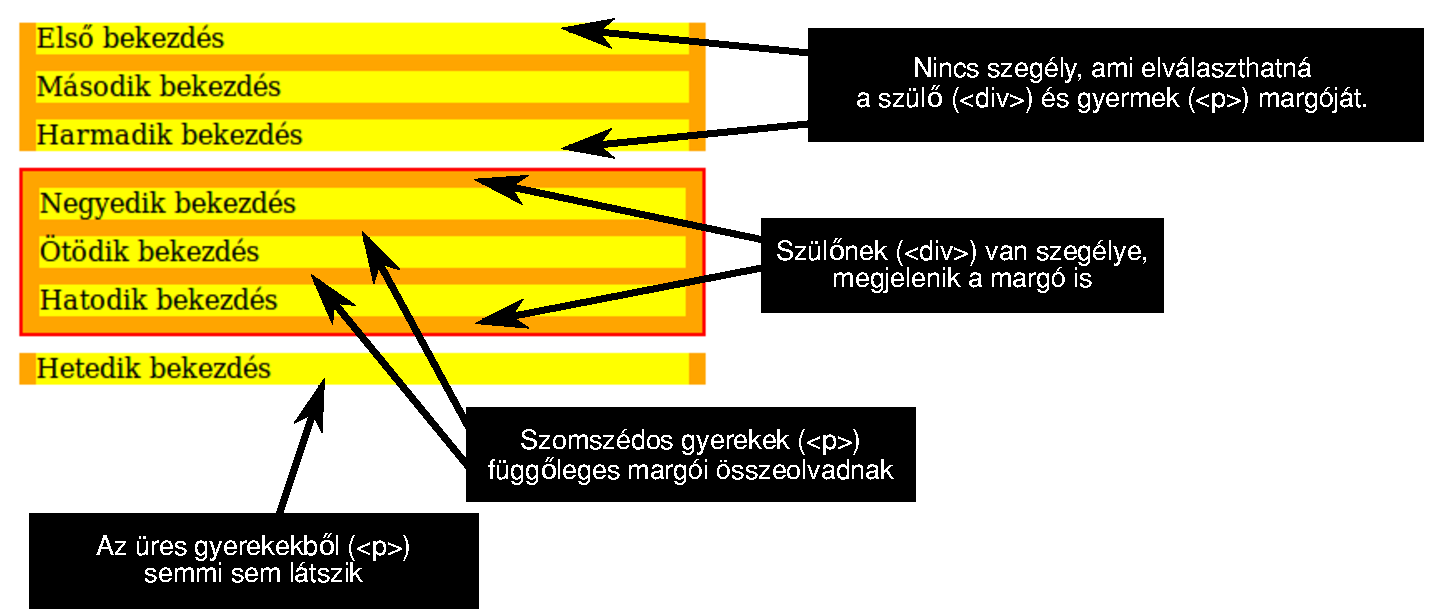
\includegraphics[scale=0.55]{margok.pdf}
  \end{center}
\end{frame}

%43
\begin{frame}
  \begin{columns}[c]
    \column{0.25\textwidth}
      Próbálja meg elkészíteni az ábrának megfelelően a dobozokat!
    \column{0.7\textwidth}
      \begin{center}
        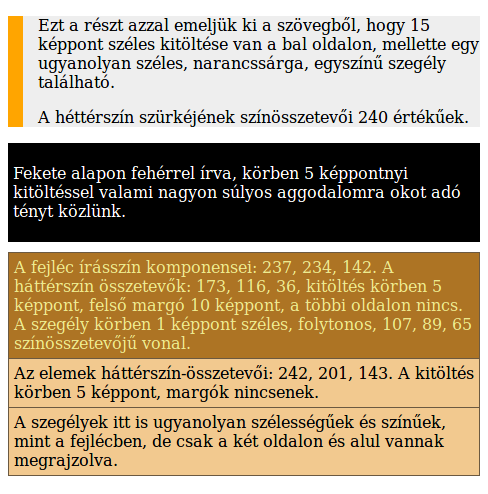
\includegraphics[scale=0.35]{dobozok.png}\\
        \textattachfile{dobozok.html}{dobozok.html}
      \end{center}
  \end{columns} 
\end{frame}

%\subsection{Kitöltés}

%47
\begin{frame}
  A kitöltések mindig átlátszók, csak a szélességük állítható:
  \begin{itemize}
    \item 1-4 érték megadásával, pl.\\
    \texttt{padding: 10px 20px 30px 40px;}\\
    (Fent, jobbra, lent, balra; további esetek mint \texttt{border-style}-nál.)
    \item Oldalakra vonatkozó tulajdonságokkal:\\
      \texttt{padding-*}, ahol \texttt{*} helyén állhat 
      \texttt{top}, \texttt{right}, \texttt{bottom}, \texttt{left}.
  \end{itemize}
\end{frame}

%48
\begin{frame}
  A kitöltés szélessége lehet:
  \begin{itemize}
    \item \texttt{inherit}: a befoglaló, szülő elem beállításait örökli
    \item CSS mértékegységgel (pl. \texttt{px}, \texttt{cm}) adott
    \item \texttt{\%}: a szülő elem méretének százaléka
  \end{itemize}
  \vfill
  Negatív értékek \kiemel{nem} használhatók.
\end{frame}

%49
\begin{frame}
  \begin{columns}[c]
    \column{0.25\textwidth}
      Próbálja meg elkészíteni az ábrának megfelelően a dobozokat!
    \column{0.7\textwidth}
      \begin{center}
        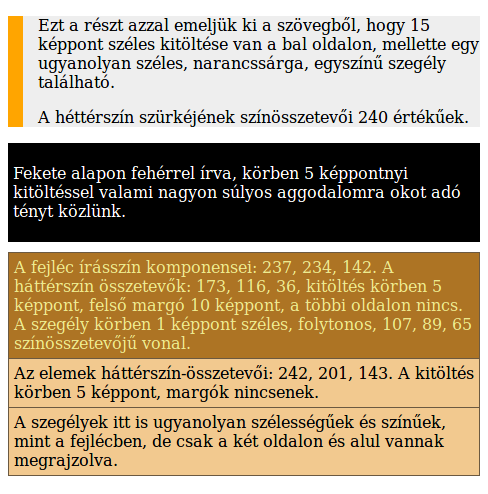
\includegraphics[scale=0.35]{dobozok.png}\\
        \textattachfile{dobozok.html}{dobozok.html}
      \end{center}
  \end{columns} 
\end{frame}

%\subsection{Körvonal}

%50
\begin{frame}
  Körvonal (outline): az elemet a szegélyen kívülről körülöleli, kiemeli környezetéből. Rálóghat más elemekre.
  \begin{description}[m]
    \item[\texttt{outline-style}] \hfill \\ Stílus, mint \texttt{border-style}, pl. \texttt{solid}, \texttt{dotted}, \texttt{double}, \dots \\A többi tulajdonság beállítása \kiemel{hatástalan} a stílus megadása nélkül!
    \item[\texttt{outline-color}] Körvonal színe. Értéke lehet \texttt{invert}, ami minden háttéren látható.
    \item[\texttt{outline-width}] Szélesség CSS mértékegységekben, vagy \texttt{thin}, \texttt{medium}, \texttt{thick}.
  \end{description}
\end{frame}

%51
\begin{frame}
  Rövidítés: 
  \begin{description}[m]
    \item[\texttt{outline: outline-width outline-style outline-color}] \hfill \\ Sorrend tetszőleges, bármelyik érték elhagyható.
  \end{description}
  \vfill
  \begin{description}[m]
    \item[\texttt{outline-offset}] \hfill \\ A körvonal távolsága a szegélytől. Ez a terület áttetsző.
  \end{description}
\end{frame}

%52
\begin{frame}
  \scriptsize
  \begin{exampleblock}{\textattachfile{korvonal.html}{korvonal.html}}
    \fontsize{7}{8} \selectfont
    \lstinputlisting[style=HTML,linerange={7-12},numbers=left,firstnumber=7]{korvonal.html}
    \lstinputlisting[style=HTML,linerange={20-23},numbers=left,firstnumber=20]{korvonal.html}
  \end{exampleblock}
  \begin{center}
    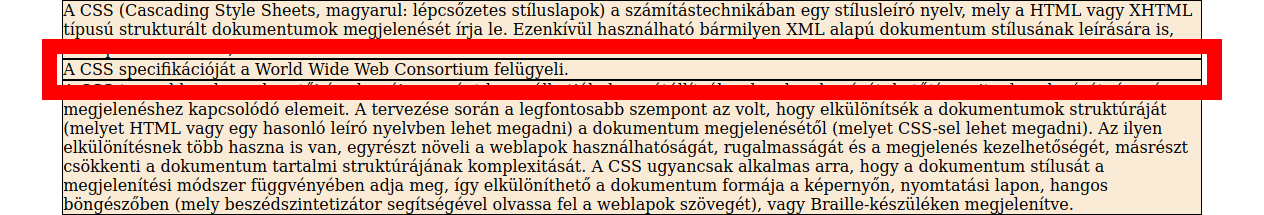
\includegraphics[width=0.9\textwidth]{korvonal.png}
  \end{center}
\end{frame}

%\subsection{Karakterkészletek}

%53
\begin{frame}
  Általános fontcsaládok: nagyon hasonló megjelenésű karakterkészletek
  \begin{description}[m]
    \item[Serif] \hfill \\ ,,Talpas'' betűkészletek; főleg bekezdések szövegéhez, mert ,,vezeti a szemet'' az alapvonalon, de képernyőn sokan nehezen olvassák
    \item[Sans-serif] \hfill \\ ,,Talp nélküli'' betűkészletek, 
    főleg címsorokhoz
    \item[Monospace] \hfill \\ ,,Egyenközű'', azonos szélességű 
    betűkből álló betűkészletek, főleg forrásszövegekhez
  \end{description}
\end{frame}

%54
\begin{frame}
  \texttt{font-family}: karakterkészlet kiválasztása
  \begin{itemize}
    \item Karakterkészletek listája; 
    ha valamelyik nincs telepítve, a következővel próbálkozik 
    $\to$ érdemes egy általános fontcsalád nevét tenni a végére
    \item Ha a névben szóköz van, idézőjelek közé kell tenni
    \item Jól bejáratott kombinációk, pl.
    \begin{itemize}
      \item \texttt{"Times New Roman", Times, serif}
      \item \texttt{Arial, Helvetica, sans-serif}
      \item \texttt{"Courier New", Courier, monospace}
    \end{itemize}
  \end{itemize}
\end{frame}

%55
\begin{frame}
  \texttt{font-style}: álló és dőlt betűk
  \begin{description}[m]
    \item[\texttt{normal}] \hfill \\ Álló betűk, alapértelmezés
    \item[\texttt{italic}] \hfill \\ Dőlt betűk
    \item[\texttt{oblique}] \hfill \\ ,,Kevésbé dőlt'', gyenge támogatás
  \end{description}
  \vfill
  \texttt{font-variant}: változatok
  \begin{description}[m]
    \item[\texttt{normal}] \hfill \\ Normál betűk, alapértelmezett.
    \item[\texttt{small-caps}] \hfill \\ Kiskapitális, a kisbetűket 
    kicsinyített nagybetűkkel helyettesíti.
  \end{description}
\end{frame}

%56
\begin{frame}
  \texttt{font-size}: méretezés
  \begin{description}[m]
    \item[Abszolút méretekben] \hfill \\ A felhasználó nem 
    méretezheti át. Pl. \texttt{px} (CSS képpont), \texttt{pt} 
    (nyomdai pont).
    \item[Relatív méretekben] \hfill \\ Felhasználó átméretezheti. Pl. \texttt{em} (1em a 
    bekezdések alapértelmezett mérete = \texttt{16px}), \texttt{\%} 
    (a szülő elem betűkészletének méretéhez viszonyítva), 
    \texttt{vw} (\texttt{1vw} = a \emph{viewport} szélességének 
    1\%-a; átméreteződik az ablak méretezésével)
    \item[Kulcsszavakkal] \hfill \\ Előre definiált méretek: \texttt{xx-small}, 
    \texttt{x-small}, \texttt{small}, \texttt{medium}, \texttt{large}, 
    \texttt{x-large}, \texttt{xx-large}. \\
    Átméretezés: \texttt{smaller}, \texttt{larger}.
  \end{description}
\end{frame}

%57
\begin{frame}
  \texttt{font-weight}: ,,vastagság'', ,,súly''
  \begin{description}[m]
    \item[\texttt{normal}] \hfill \\ Normál szélesség (400), alapértelmezett.
    \item[\texttt{bold}] \hfill \\ Félkövér (700)
    \item[\texttt{bolder}, \texttt{lighter}] \hfill \\ Növeli, 
    csökkenti a vastagságot
    \item[\texttt{100, 200, 300, \dots, 900}] \hfill \\ Különféle 
    vastagságok, de többnyire csak a normál és a félkövér támogatott.
  \end{description}
\end{frame}

%58
\begin{frame}
  Rövidítés:
  \begin{description}[m]
    \item[\texttt{font: font-style font-variant font-weight 
    font-size/line-height}] \hfill \\
    \item[\qquad \texttt{font-family | caption | icon | menu | 
    message-box | }] \hfill \\
    \item[\qquad \texttt{small-caption | status-bar | initial | inherit;}] \hfill \\ A méret és a 
    karakterkészlet megadása kötelező. A \texttt{caption}, 
    \texttt{icon}, ... kulcsszavakkal lehet a böngésző által 
    valamilyen célra már használt beállításokat kérni egy adott helyen.
  \end{description}
\end{frame}

%59
\begin{frame}
  \begin{exampleblock}{\textattachfile{karakter.html}{karakter.html}}
    \fontsize{7}{8} \selectfont
    \lstinputlisting[style=HTML,linerange={6-10},numbers=left,firstnumber=6]{karakter.html}
    \lstinputlisting[style=HTML,linerange={13-25},numbers=left,firstnumber=13]{karakter.html}
  \end{exampleblock}
\end{frame}

%60
\begin{frame}
  \begin{center}
    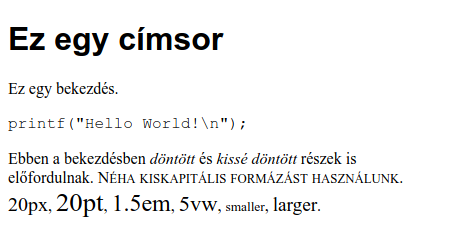
\includegraphics[scale=0.6]{karakter.png}
  \end{center}
\end{frame}

%61
\begin{frame}
  Karakterkészletek letölthetők a hálózatról: \texttt{@font-face}
  \begin{itemize}
    \item egyedi megjelenést kölcsönöz
    \item mindenki ugyanazt a készletet használja, garantáltan azonos megjelenés mindenhol (sok eszközön hiányosak a készletek, főleg a ritkán használt karakterek)
  \end{itemize}
  \vfill
  Megbízhatóan használható formátumok:
  \begin{itemize}
    \item \hiv{\href{https://en.wikipedia.org/wiki/TrueType}{TrueType Font (TTF)}}
    \item \hiv{\href{https://en.wikipedia.org/wiki/OpenType}{OpenType Font (OTF)}}
    \item \hiv{\href{https://en.wikipedia.org/wiki/Web_Open_Font_Format}{Web Open Font Format (WOFF)}}
  \end{itemize}
\end{frame}

%62
\begin{frame}
  A \texttt{@font-face} szabályban használható tulajdonságok:
  \begin{description}[m]
    \item[\texttt{font-family}] \hfill \\ Ezzel a névvel lehet majd hivatkozni a karakterkészletre később, kötelező.
    \item[\texttt{src}] \hfill \\ A fájl forrását adja meg \texttt{url()} CSS függvénnyel, kötelező.
    \item[\texttt{font-stretch}] \hfill \\ Ha a karakterkészletnek készültek különféle sűrűségű változatai, ezzel lehet kiválasztani, hogy valamelyiket milyennek tekintsen a böngésző (pl. \texttt{normal}, \texttt{condensed}, \texttt{expanded}). Ennek hiányában a böngészőnek kell előállíttatnia a speciális formákat a normálból kiindulva.
    \item[\texttt{font-style}] \hfill \\ Hasonlóan, dőlt változatokhoz (pl. \texttt{normal}, \texttt{italic}).
    \item[\texttt{font-weight}] \hfill \\ Hasonlóan, a ,,kövérséghez'' (pl. \texttt{normal}, \texttt{bold}).
  \end{description}
\end{frame}

%63
\begin{frame}
  \begin{columns}[c]
    \column{0.65\textwidth}
      \begin{exampleblock}{\textattachfile{webfont.html}{webfont.html}}
        \fontsize{7}{8} \selectfont
        \lstinputlisting[style=HTML,linerange={7-17},numbers=left,firstnumber=7]{webfont.html}
        \lstinputlisting[style=HTML,linerange={21-22},numbers=left,firstnumber=21]{webfont.html}
      \end{exampleblock}
    \column{0.3\textwidth}
      
\includegraphics[width=\textwidth]{webfont.png}
  \end{columns}
\end{frame}

%64
\begin{frame}
  \hiv{\href{https://developers.google.com/fonts}{Google Fonts}}
  \begin{itemize}
    \item Több száz ingyenes karakterkészlet
    \item Könnyű kereshetőség
    \item Egyszerű integráció a weboldalba
  \end{itemize}
\end{frame}

%65
\begin{frame}
  \begin{columns}[c]
    \column{0.65\textwidth}
      \begin{exampleblock}{\textattachfile{googleFonts.html}{googleFonts.html}}
        \scriptsize
        \lstinputlisting[style=HTML,linerange={6-12},numbers=left,firstnumber=6]{googleFonts.html}
        \lstinputlisting[style=HTML,linerange={15-15},numbers=left,firstnumber=15]{googleFonts.html}
      \end{exampleblock}
    \column{0.3\textwidth}
      
\includegraphics[width=\textwidth]{googleFonts.png}
  \end{columns}
\end{frame}

%66
\begin{frame}
  \begin{columns}[c]
    \column{0.5\textwidth}
      Készítse el Semmelweis Ignác oldalát a \hiv{\href{https://hu.wikipedia.org/wiki/Semmelweis_Ign\%C3\%A1c}{Wiki}} oldal szövegét felhasználva!
      \begin{itemize}
        \item Töltse le a \hiv{\href{https://befonts.com/ballerina-script-font.html}{Ballerina}} karakterkészletet!
        \item Használja ezt az első szintű címsorban szereplő név kiírására, 42 nyomdai pont méretben!
        \item A bekezdések szövegét írja \hiv{\href{https://fonts.google.com/}{Libre Baskerville}} karakterkészlettel, 12 nyodai pont mérettel!
        \item Készítsen stílusokat a félkövér és dőlt betűs részek megjelöléséhez!
      \end{itemize}
    \column{0.45\textwidth}
      \begin{exampleblock}{\textattachfile{semmelweis.html}{semmelweis.html}}
        \begin{center}
          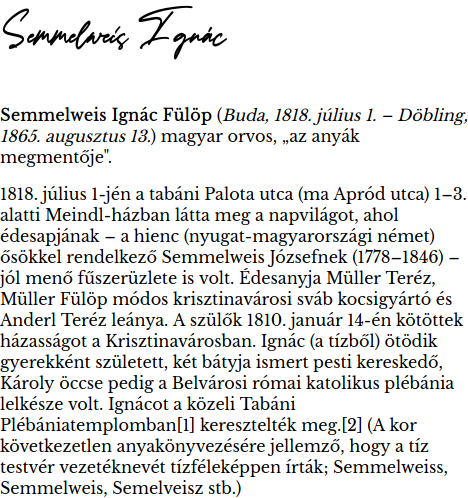
\includegraphics[width=0.7\textwidth]{semmelweis.png}
        \end{center}
      \end{exampleblock}
  \end{columns}
\end{frame}

% önálló feladat

%\subsection{Szövegformázás}

%53
\begin{frame}
  \begin{description}[m]
    \item[\texttt{text-align}] \hfill \\ Vízszintes igazítás: \texttt{left} (balra), \texttt{center} (középre), \texttt{right} (jobbra), \texttt{justify} (sorkizárt)
  \end{description}
  \begin{columns}[c]
    \column{0.6\textwidth}
      \begin{exampleblock}{\textattachfile{vizszintes.html}{vizszintes.html}}
        \tiny
        \lstinputlisting[style=HTML,linerange={7-10},numbers=left,firstnumber=7]{vizszintes.html}
        \lstinputlisting[style=HTML,linerange={15-16},numbers=left,firstnumber=15]{vizszintes.html}
      \end{exampleblock}
    \column{0.35\textwidth}
      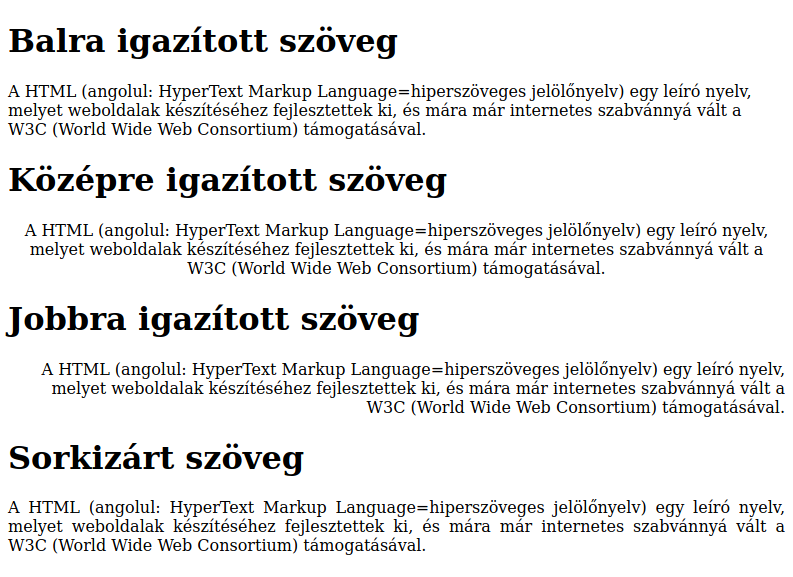
\includegraphics[width=\textwidth]{vizszintes.png}
  \end{columns}
\end{frame}

%54
\begin{frame}
  \texttt{hyphens}: elválasztások, hogy a szöveg tördelése még finomabb legyen
  \begin{description}[m]
    \item[\texttt{none}] \hfill \\ nincs elválasztás, alapértelmezés
    \item[\texttt{manual}] \hfill \\ elválasztás csak a kézzel előre megjelölt helyeken (\texttt{\&hyphen;}, \texttt{\&shy;})
    \item[\texttt{auto}] \hfill \\ automatikus elválasztás
  \end{description}
\end{frame}

%55
\begin{frame}
  \begin{exampleblock}{\textattachfile{elvalasztas.html}{elvalasztas.html}}
    \scriptsize
    \lstinputlisting[style=HTML,linerange={8-8},numbers=left,firstnumber=8]{elvalasztas.html}
    \lstinputlisting[style=HTML,linerange={12-13},numbers=left,firstnumber=12]{elvalasztas.html}
    \lstinputlisting[style=HTML,linerange={16-16},numbers=left,firstnumber=16]{elvalasztas.html}
  \end{exampleblock}
  \begin{center}
    
\includegraphics[width=\textwidth]{elvalasztas.png}
  \end{center}
\end{frame}

%56
\begin{frame}
  \texttt{vertical-align}: tetszőleges elem függőleges igazítása
  \begin{description}[m]
    \item[\texttt{baseline}] \hfill \\ szülő szövegének alapvonalához
    \item[\emph{távolság}] \hfill \\ tetszőleges mértékű süllyesztéshez/emeléshez, negatív érték is elfogadott
    \item[\texttt{\%}] \hfill \\ sormagasság \%-ában megadott emelés/süllyesztés, negatív érték is elfogadott
    \item[\texttt{sub}] \hfill \\ szülő alsó indexéhez
    \item[\texttt{super}] \hfill \\ szülő felső indexéhez
  \end{description}
\end{frame}

%57
\begin{frame}
  \begin{description}[m]
    \item[\texttt{top}] \hfill \\ sor legmagasabb eleméhez
    \item[\texttt{text-top}] \hfill \\ szülő elem szövegének tetejéhez
    \item[\texttt{middle}] \hfill \\ szülő közepéhez
    \item[\texttt{bottom}] \hfill \\  sor legalsó eleméhez
    \item[\texttt{text-bottom}] \hfill \\ szülő szövegének aljához
  \end{description}
\end{frame}

%58
\begin{frame}
  \begin{columns}[c]
    \column{0.55\textwidth}
      \begin{exampleblock}{\textattachfile{fuggoleges.html}{fuggoleges.html}}
        \tiny
        \lstinputlisting[style=HTML,linerange={7-9},numbers=left,firstnumber=7]{fuggoleges.html}
        \lstinputlisting[style=HTML,linerange={13-15},numbers=left,firstnumber=13]{fuggoleges.html}
      \end{exampleblock}
    \column{0.4\textwidth}
      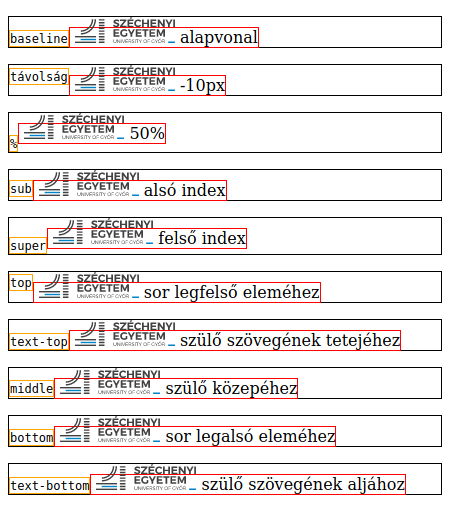
\includegraphics[width=\textwidth]{fuggoleges.png}
  \end{columns}
\end{frame}

%59
\begin{frame}
  \begin{description}[m]
    \item[\texttt{text-indent}] \hfill \\ Első sor behúzása: \emph{távolság} (a bekezdés bal szélétől számított behúzás), \texttt{\%} (szülő elem szélességének százalékában adott behúzás)
  \end{description}
  \begin{columns}[c]
    \column{0.6\textwidth}
      \begin{exampleblock}{\textattachfile{behuzas.html}{behuzas.html}}
        \tiny
        \lstinputlisting[style=HTML,linerange={7-10},numbers=left,firstnumber=7]{behuzas.html}
        \lstinputlisting[style=HTML,linerange={14-16},numbers=left,firstnumber=14]{behuzas.html}
      \end{exampleblock}
    \column{0.35\textwidth}
      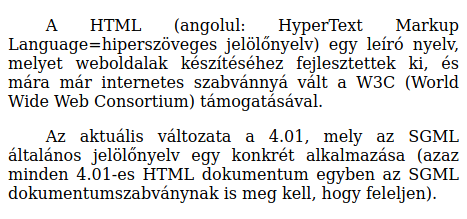
\includegraphics[width=\textwidth]{behuzas.png}
  \end{columns}
\end{frame}

%60
\begin{frame}
  \texttt{white-space}: fehér karakterek értelmezése
  \begin{description}[m]
    \item[\texttt{normal}] \hfill \\ szomszédos fehér karaktereket összevonja, alapértelmezés
    \item[\texttt{nowrap}] \hfill \\ nem tördeli a hosszú sorokat, de a szomszédos fehér karaktereket összevonja
    \item[\texttt{pre}] \hfill \\ utánozza a \texttt{<pre>} HTML elem működését, minden fehér karaktert megőriz
    \item[\texttt{pre-line}] \hfill \\ szomszédos fehér karaktereket összevonja, de tördeli a sorokat, ha szükséges
    \item[\texttt{pre-wrap}] \hfill \\ minden fehér karaktert megőriz, és tördel, ha szükséges
  \end{description}
\end{frame}

%61
\begin{frame}
  Nem választ magától \texttt{monospace} karakterkészletet!
  \begin{columns}[c]
    \column{0.6\textwidth}
      \begin{exampleblock}{\textattachfile{fahrcels2.html}{fahrcels2.html}}
        \footnotesize
        \lstinputlisting[style=HTML,linerange={7-10},numbers=left,firstnumber=7]{fahrcels2.html}
        \lstinputlisting[style=HTML,linerange={14-16},numbers=left,firstnumber=14]{fahrcels2.html}
      \end{exampleblock}
    \column{0.35\textwidth}
      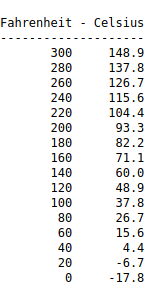
\includegraphics[width=0.7\textwidth]{fahrcels2.png}
  \end{columns}
\end{frame}

%62
\begin{frame}
  \texttt{letter-spacing}: betűk közötti távolság
  \begin{description}[m]
    \item[\texttt{normal}] \hfill \\ szokásos távolság, alapértelmezés
    \item[\emph{távolság}] \hfill \\ betűk közötti távolság, negatív érték is elfogadott
  \end{description}
  \vfill
  \texttt{word-spacing}: szavak közötti távolság
  \begin{description}[m]
    \item[\texttt{normal}] \hfill \\ szokásos távolság (betűmagasság negyede), alapértelmezés
    \item[\emph{távolság}] \hfill \\ szavak közötti távolság, negatív érték is elfogadott
  \end{description}
\end{frame}

%63
\begin{frame}
  \begin{exampleblock}{\textattachfile{tavolsag.html}{tavolsag.html}}
    \footnotesize
    \lstinputlisting[style=HTML,linerange={7-11},numbers=left,firstnumber=7]{tavolsag.html}
    \lstinputlisting[style=HTML,linerange={15-16},numbers=left,firstnumber=15]{tavolsag.html}
  \end{exampleblock}
  \begin{center}
    
\includegraphics[width=0.8\textwidth]{tavolsag.png}
  \end{center}
\end{frame}

%64
\begin{frame}
  \texttt{text-transform}: szöveg átalakítása
  \begin{description}[m]
    \item[\texttt{normal}] \hfill \\ nincs átalakítás, alapértelmezés
    \item[\texttt{capitalize}] \hfill \\ minden kezdőbetűt nagybetűvel nyomtat
    \item[\texttt{uppercase}] \hfill \\ csupa nagybetűvel nyomtat
    \item[\texttt{lowercase}] \hfill \\ csupa kisbetűvel nyomtat
  \end{description}
\end{frame}

%65
\begin{frame}
  \begin{exampleblock}{\textattachfile{nagybetu.html}{nagybetu.html}}
    \scriptsize
    \lstinputlisting[style=HTML,linerange={7-9},numbers=left,firstnumber=7]{nagybetu.html}
    \lstinputlisting[style=HTML,linerange={13-14},numbers=left,firstnumber=13]{nagybetu.html}
  \end{exampleblock}
  \begin{center}
    
\includegraphics[scale=0.5]{nagybetu.png}
  \end{center}
\end{frame}

%66
\begin{frame}
  \texttt{text-decoration-line}: vonal húzása a szöveggel párhuzamosan
  \begin{description}[m]
    \item[\texttt{none}] \hfill \\ nincs vonalazás, alapértelmezés. Pl. hivatkozások aláhúzásának eltávolításához használható.
    \item[\texttt{underline}] \hfill \\ aláhúzza a szöveget; \kiemel{félrevezetheti az olvasót}, ha nem csak a hivatkozások jelennek meg aláhúzással!
    \item[\texttt{overline}] \hfill \\ a szöveg fölött húz vonalat
    \item[\texttt{line-through}] \hfill \\ áthúzza a szöveget
  \end{description}
\end{frame}

%67
\begin{frame}
  \texttt{text-decoration-style}: a vonal stílusa
  \begin{description}[m]
    \item[\texttt{solid}] \hfill \\ folytonos vonal
    \item[\texttt{double}] \hfill \\ dupla vonal
    \item[\texttt{dotted}] \hfill \\ pontvonal
    \item[\texttt{dashed}] \hfill \\ szaggatott vonal
    \item[\texttt{wavy}] \hfill \\ hullámos vonal
  \end{description}
\end{frame}

%68
\begin{frame}
  \texttt{text-decoration-color}: a vonal színe
  \begin{description}[m]
    \item[\emph{szín}] \hfill \\ tetszőleges CSS színmegadási móddal
  \end{description}
  \vfill
  Rövidítés:
  \begin{description}[m]
    \item[\texttt{text-decoration:}]
    \item[\qquad\texttt{text-decoration-line text-decoration-color text-decoration-style}] \hfill \\ Akár többféle vonal is megadható, tetszőleges rész elhagyható, sorrend tetszőleges
  \end{description}
\end{frame}

%69
\begin{frame}
  \begin{exampleblock}{\textattachfile{dekoracio.html}{dekoracio.html}}
    \footnotesize
    \lstinputlisting[style=HTML,linerange={7-11},numbers=left,firstnumber=7]{dekoracio.html}
    \lstinputlisting[style=HTML,linerange={15-17},numbers=left,firstnumber=15]{dekoracio.html}
  \end{exampleblock}
  \begin{center}
    
\includegraphics[width=\textwidth]{dekoracio.png}
  \end{center}
\end{frame}

%70
\begin{frame}
  \texttt{text-shadow}: szöveg árnyéka
  \begin{description}[m]
    \item[\texttt{h-shadow v-shadow blur-radius color}] \hfill \\ vízszintes eltolás, függőleges eltolás, elmosás mértéke, szín. \\ Az elmosás mértéke elhagyható, a többi kötelező. Az eltolásoknál negatív értékek megengedettek. Vesszővel elválasztva több árnyék is megadható egyszerre.
    \item[\texttt{none}] nincs árnyék, alapértelmezés
  \end{description}
\end{frame}

%71
\begin{frame}
  \begin{columns}[c]
    \column{0.7\textwidth}
      \begin{exampleblock}{\textattachfile{arnyek.html}{arnyek.html}}
        \scriptsize
        \lstinputlisting[style=HTML,linerange={7-12},numbers=left,firstnumber=7]{arnyek.html}
        \lstinputlisting[style=HTML,linerange={16-18},numbers=left,firstnumber=16]{arnyek.html}
      \end{exampleblock}
    \column{0.25\textwidth}
      
\includegraphics[width=\textwidth]{arnyek.png}
  \end{columns}
\end{frame}

%72
\begin{frame}
  \texttt{line-height}: sormagasság
  \begin{description}[m]
    \item[\texttt{normal}] \hfill \\ betűméretből következő sormagasság, alapértelmezett
    \item[\emph{szám}] \hfill \\ az aktuális betűméretet ezzel szorozva kapja meg a sormagasságot
    \item[\emph{távolság}] \hfill \\ rögzített sormagasság, CSS mértékegységben
    \item[\texttt{\%}] \hfill \\ az aktuális betűméret \%-a
  \end{description}
\end{frame}

%73
\begin{frame}
  \begin{columns}[c]
    \column{0.65\textwidth}
      \begin{exampleblock}{\textattachfile{sormagassag.html}{sormagassag.html}}
        \scriptsize
        \lstinputlisting[style=HTML,linerange={7-9},numbers=left,firstnumber=7]{sormagassag.html}
        \lstinputlisting[style=HTML,linerange={13-15},numbers=left,firstnumber=13]{sormagassag.html}
      \end{exampleblock}
    \column{0.3\textwidth}
      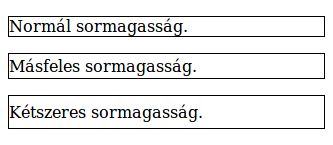
\includegraphics[width=\textwidth]{sormagassag.png}
  \end{columns}
\end{frame}

%74
\begin{frame}
  Többféle írásirány támogatott egyazon oldalon
  \begin{columns}[c]
    \column{0.65\textwidth}
      \begin{exampleblock}{\textattachfile{irasirany.html}{irasirany.html}}
        \footnotesize
        \lstinputlisting[style=HTML,linerange={7-10},numbers=left,firstnumber=7]{irasirany.html}
        \lstinputlisting[style=HTML,linerange={14-15},numbers=left,firstnumber=14]{irasirany.html}
      \end{exampleblock}
    \column{0.3\textwidth}
      
\includegraphics[width=\textwidth]{irasirany.png}
  \end{columns}  
\end{frame}

%75
\begin{frame}
  \begin{columns}[c]
    \column{0.5\textwidth}
      \footnotesize
      Készítse el az ábrán látható weboldalt!
      \begin{itemize}
        \item Induljon ki a \textattachfile{szoveg.txt}{szoveg.txt} fájlból!
        \item A címsor betűi között hagyjon 5-5 képpontnyi helyet,
        \item írja csupa nagybetűvel, és
        \item jelenítsen meg alatta 3-3 képpontnyival jobbra és lefelé eltolt árnyékot, mely kék színű, és elmosásának sugara 10 képpont!
        \item A bekezdés legyen sorkizárt igazítású, 
        \item a sormagasság másfélszeres,
        \item az első sor behúzása 20 képpontnyi,
        \item és automatikusan elválasztott!
        \item Az emberek neveit emelje ki zöld színű, dupla aláhúzással!
      \end{itemize}
    \column{0.45\textwidth}
      \begin{exampleblock}{\textattachfile{szoveg.html}{szoveg.html}}
        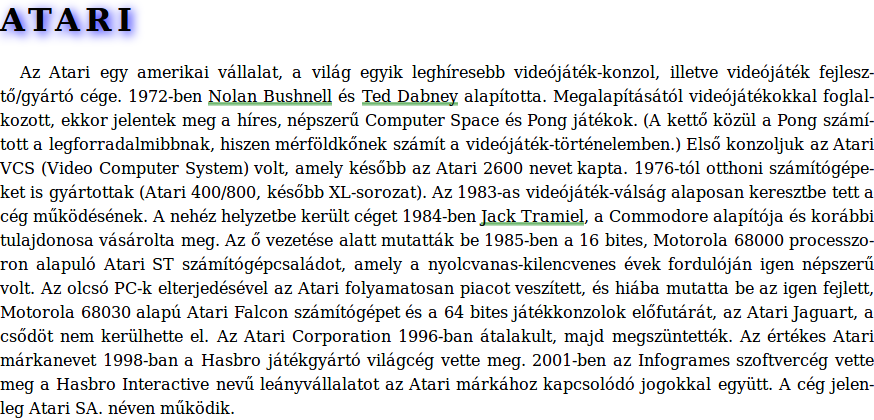
\includegraphics[width=\textwidth]{szoveg.png}
      \end{exampleblock}
  \end{columns}
\end{frame}

\subsection{Hivatkozások}

%_
\begin{frame}
  A \emph{látszólagos osztály} (pseudo class) egy, a szelektor utáni 
  :-ot követő kulcsszó, amivel a kiválasztott elem(ek) különféle 
  állapotaiban alkalmazandó formázás adható meg.\\
  \vfill
  \hiv{\href{https://developer.mozilla.org/en-US/docs/Web/CSS/Pseudo-classes}{Látszólagos osztályok referenciája}}
  \vfill
  Hivatkozásoknál alkalmazható:
  \begin{description}[m]
    \item[\texttt{link}] \hfill \\ Még nem követték a hivatkozást
    \item[\texttt{visited}] \hfill \\ Már követték a hivatkozást
    \item[\texttt{hover}] \hfill \\ Egér a hivatkozás felett
    \item[\texttt{active}] \hfill \\ Már rákattintottak, de az új 
    tartalom még nem töltődött be
  \end{description}
  \kiemel{Ebben a sorrendben} kell definiálni őket!
\end{frame}

%
\begin{frame}
  \begin{exampleblock}{\textattachfile{hivatkozas.html}{hivatkozas.html}}
    \scriptsize
    \lstinputlisting[style=HTML,linerange={7-10},numbers=left,firstnumber=7]{hivatkozas.html}
    \lstinputlisting[style=HTML,linerange={14-16},numbers=left,firstnumber=14]{hivatkozas.html}
  \end{exampleblock}
  \begin{center}
    
\includegraphics[width=0.8\textwidth]{hivatkozas.png}
  \end{center}
\end{frame}

%ide jöjjenek a felsorolások
\subsection{Táblázatok}

%_
\begin{frame}
  \begin{columns}[c]
    \column{0.5\textwidth}
      Táblázatok alapértelmezett formázása:
      \begin{itemize}
        \item Cellaméretek a tartalomhoz igazodnak
        \item Nincsenek szegélyek
        \item Fejléc (\texttt{<th>}) cellák félkövérek, középre zártak
        \item Normál cellák (\texttt{<td>}) balra zártak
      \end{itemize}
    \column{0.45\textwidth}
        \begin{exampleblock}{\textattachfile{tablazat01.html}{tablazat01.html}}
          \begin{center}
            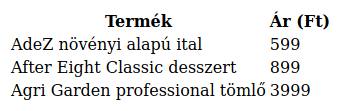
\includegraphics[width=\textwidth]{tablazat01.png}
          \end{center}
        \end{exampleblock}
  \end{columns}
\end{frame}

%_
\begin{frame}
  Kaphat szegélyt a teljes táblázat \dots
  \begin{columns}[c]
    \column{0.66\textwidth}
      \begin{exampleblock}{\textattachfile{tablazat02.html}{tablazat02.html}}
        \scriptsize
        \lstinputlisting[style=HTML,linerange={7-7},numbers=left,firstnumber=7]{tablazat02.html}
        \lstinputlisting[style=HTML,linerange={11-16},numbers=left,firstnumber=11]{tablazat02.html}
      \end{exampleblock}
    \column{0.3\textwidth}
      \includegraphics[width=\textwidth]{tablazat02.png}
  \end{columns}
\end{frame}

%_
\begin{frame}
  \dots vagy annak cellái \dots
  \vfill
  \begin{exampleblock}{\textattachfile{tablazat03.html}{tablazat03.html}}
    \lstinputlisting[style=HTML,linerange={7-7},numbers=left,firstnumber=7]{tablazat03.html}
  \end{exampleblock}
  \begin{center}
    \includegraphics[width=0.4\textwidth]{tablazat03.png}
  \end{center}
\end{frame}

%_
\begin{frame}
  \dots vagy mindkettő.
  \vfill
  \begin{exampleblock}{\textattachfile{tablazat04.html}{tablazat04.html}}
    \lstinputlisting[style=HTML,linerange={7-7},numbers=left,firstnumber=7]{tablazat04.html}
  \end{exampleblock}
  \begin{center}
    \includegraphics[width=0.4\textwidth]{tablazat04.png}
  \end{center}
\end{frame}

%_
\begin{frame}
  A cellák közötti távolság változtatható a \texttt{<table>} \texttt{border-spacing} tulajdonságával \dots
  \vfill
  \begin{exampleblock}{\textattachfile{tablazat05.html}{tablazat05.html}}
    \lstinputlisting[style=HTML,linerange={7-8},numbers=left,firstnumber=7]{tablazat05.html}
  \end{exampleblock}
  \begin{center}
    \includegraphics[width=0.4\textwidth]{tablazat05.png}
  \end{center}
\end{frame}

%_
\begin{frame}
  \dots de teljesen el is tüntethető a \texttt{<table>} \texttt{border-collapse} tulajdonságával:
  \begin{description}[m]
    \item[\texttt{separate}] elkülönített cellák, alapértelmezés.
    \item[\texttt{collapse}] összevont cellaszegélyek.
  \end{description}
  \vfill
  \begin{exampleblock}{\textattachfile{tablazat06.html}{tablazat06.html}}
    \lstinputlisting[style=HTML,linerange={7-8},numbers=left,firstnumber=7]{tablazat06.html}
  \end{exampleblock}
  \begin{center}
    \includegraphics[width=0.4\textwidth]{tablazat06.png}
  \end{center}
\end{frame}

%_
\begin{frame}
  A cellák szegélye és tartalma közötti távolság a \texttt{<td>}, \texttt{<th>} \texttt{padding} tulajdonságával állítható.
  \begin{exampleblock}{\textattachfile{tablazat07.html}{tablazat07.html}}
    \footnotesize
    \lstinputlisting[style=HTML,linerange={7-11},numbers=left,firstnumber=7]{tablazat07.html}
  \end{exampleblock}
  \begin{center}
    \includegraphics[width=0.4\textwidth]{tablazat07.png}
  \end{center}
\end{frame}

%_
\begin{frame}
  A cellákon belüli igazítás a \texttt{text-align}, \texttt{vertical-align} tulajdonságokkal állítható.
  \begin{exampleblock}{\textattachfile{tablazat08.html}{tablazat08.html}}
    \scriptsize
    \lstinputlisting[style=HTML,linerange={7-13},numbers=left,firstnumber=7]{tablazat08.html}
  \end{exampleblock}
  \begin{center}
    \includegraphics[width=0.35\textwidth]{tablazat08.png}
  \end{center}
\end{frame}

%_
\begin{frame}
  Ha a táblázat szélesebb, mint amit a tartalom indokol, a maradék hely arányosan lesz elosztva.
  \begin{exampleblock}{\textattachfile{tablazat09.html}{tablazat09.html}}
    \scriptsize
    \lstinputlisting[style=HTML,linerange={7-14},numbers=left,firstnumber=7]{tablazat09.html}
  \end{exampleblock}
  \begin{center}
    \includegraphics[width=\textwidth]{tablazat09.png}
  \end{center}
\end{frame}

%_
\begin{frame}
  \begin{columns}[c]
    \column{0.3\textwidth}
      \small
      Az olvashatóság javításához pl. kiemelhetjük az egér alatti sort a \texttt{:hover} látszólagos osztállyal.\\
      Figyeljük meg a ,,csíkozást''!
      \vfill
      \begin{center}
        \includegraphics[width=\textwidth]{tablazat10.png}
      \end{center}
    \column{0.66\textwidth}
      \begin{exampleblock}{\textattachfile{tablazat10.html}{tablazat10.html}}
        \scriptsize
        \lstinputlisting[style=HTML,linerange={7-14},numbers=right,firstnumber=7]{tablazat10.html}
      \end{exampleblock}
  \end{columns}
\end{frame}

%_
\begin{frame}
  Az olvashatóság a sorok váltakozó háttérszínével is javítható. Egy szülő elem (pl. \texttt{<table>}) gyerekei (sorok) közül meghatározottak kiválasztása: \hiv{\href{https://developer.mozilla.org/en-US/docs/Web/CSS/:nth-child}{\texttt{nth-child()}}} látszólagos osztállyal.
  \begin{columns}[c]
    \column{0.66\textwidth}
      \begin{description}[m]
        \item[\texttt{An+b}] \hfill \\ $n = 0 \dots$, de a gyerekek számozása 1-től indul!
        \item[\texttt{even}] \hfill \\ Páros elemek $\equiv$ \texttt{2n}
        \item[\texttt{odd}] \hfill \\ Páratlan elemek $\equiv$ \texttt{2n+1}
      \end{description}
    \column{0.3\textwidth}
      \includegraphics[width=\textwidth]{tablazat11.png}
  \end{columns} 
\end{frame}

%_
\begin{frame}
  \begin{exampleblock}{\textattachfile{tablazat11.html}{tablazat11.html}}
    \small
    \lstinputlisting[style=HTML,linerange={7-17},numbers=left,firstnumber=7]{tablazat11.html}
  \end{exampleblock}
\end{frame}

%_
\begin{frame}
  \begin{columns}[c]
    \column{0.66\textwidth}
      Görgethető táblázat, trükkök:
      \begin{itemize}
        \item Rögzített fejléc $\to$ két külön táblázat, csak az alsó görgethető
        \item Görgetés: táblázat beágyazva egy túl alacsony elembe, és \texttt{overflow-y: scroll} (hasonlóan a vízszintes irányú görgetés is lehetséges az \texttt{overflow-x} tulajdonsággal)
        \item Legyenek a két táblázat oszlopai rendre azonos szélességűek!
      \end{itemize}
    \column{0.3\textwidth}
      \includegraphics[width=\textwidth]{tablazat12.png}
  \end{columns}
\end{frame}

%_
\begin{frame}
  \begin{exampleblock}{\textattachfile{tablazat12.html}{tablazat12.html}}
    \fontsize{7}{8} \selectfont
    \lstinputlisting[style=HTML,linerange={28-41},numbers=left,firstnumber=28]{tablazat12.html}
    \lstinputlisting[style=HTML,linerange={51-53},numbers=left,firstnumber=51]{tablazat12.html}
  \end{exampleblock}
\end{frame}

%_
\begin{frame}
  \begin{exampleblock}{\textattachfile{tablazat12.html}{tablazat12.html}}
    \fontsize{7}{8} \selectfont
    \lstinputlisting[style=HTML,linerange={7-24},numbers=left,firstnumber=7]{tablazat12.html}
  \end{exampleblock}
\end{frame}

%_
\begin{frame}
  Táblázat címkéjének elhelyezése: \texttt{caption-side}
  \begin{description}[m]
    \item[\texttt{top}] \hfill \\ Fent, alapértelmezés.
    \item[\texttt{bottom}] \hfill \\ Lent.
  \end{description}
  \vfill
  Üres cellák szegélyeinek rajzolása: \texttt{empty-cells}
  \begin{description}[m]
    \item[\texttt{show}] \hfill \\ Megrajzolja, alapértelmezés.
    \item[\texttt{hide}] \hfill \\ Nem rajzolja meg.
  \end{description}
\end{frame}

%_
\begin{frame}
  Táblázat megjelenítési algoritmus: \texttt{table-layout}
  \begin{description}[m]
    \item[\texttt{auto}] \hfill \\ A cellák szélessége a legszélesebb nem tördelhető tartalmi elem függvénye. Alapértelmezés.
    \item[\texttt{fixed}] \hfill \\ Az oszlopok szélességét vagy
    \begin{itemize}
      \item a \texttt{<table>} és \texttt{<col>} elemek szélességei adják meg, vagy
      \item az első sor celláinak szélességei. Ha ilyen nincs, egyforma szélesek lesznek a cellák.
    \end{itemize}
    Nagy táblázatoknál jelentősen gyorsabb megjelenés.
  \end{description}
\end{frame}

%_
\begin{frame}
  Készítse el a \textattachfile{queen.png}{queen.png} fájl felhasználásával az alábbi weboldalt, ami a \hiv{\href{https://hu.wikipedia.org/wiki/Nyolckir\%C3\%A1lyn\%C5\%91-probl\%C3\%A9ma}{Nyolckirálynő probléma}} egy lehetséges megoldását mutatja! Ügyeljen rá, hogy keskeny kijelzőkön a táblázat vízszintesen görgethető legyen! (A cellák 50x50, a képek 40x40px méretűek.)
  \begin{exampleblock}{\textattachfile{sakk.html}{sakk.html}}
    \begin{center}
      \includegraphics[scale=0.15]{sakk1.png}\hspace{1cm}
      \includegraphics[scale=0.15]{sakk2.png}
    \end{center}
  \end{exampleblock}  
\end{frame}


\end{document}
